\documentclass[12pt,a4paper]{article}

\makeatletter
\def\input@path{{/home/maenwe/Master_CSM/modèle_cours_latex}}
\makeatother

\usepackage{prise_de_note}


\usepackage{graphicx}
\graphicspath{{Image/}}

\begin{document}
	
	\begin{titlepage}
		\centering
		
		% Logo
		\begin{figure}[h]
			\centering
			% Ajustez la largeur si besoin (ex: 0.4 ou 0.6)
			
\includegraphics[width=0.5\textwidth]{logo.jpg} 
		\end{figure}
		
		\vspace{2cm}
		
		% Filet horizontal du haut
		\rule{\linewidth}{0.5mm} \\[0.4cm]
		
		% Titre
		{\color{bleuTitre} \Huge \bfseries Projet Tutoré} \\[0.4cm]
		
		% Filet horizontal du bas
		\rule{\linewidth}{0.5mm}
		
		\vspace{1.5cm}
		
		{\Large Étude de la chute de Phobos sur Mars}
		
		\vfill
		
		% Bloc Informations
		\begin{minipage}{0.45\textwidth}
			\begin{flushleft} \large
				\textbf{Encadrant :} \\
				Mariko \textsc{DUNSEATH}
			\end{flushleft}
		\end{minipage}
		\hfill
		\begin{minipage}{0.45\textwidth}
			\begin{flushright} \large
				\textbf{Étudiant :} \\
				Armand \textsc{DELLACHERIE}\\
				Nathan \textsc{HASCOET}
			\end{flushright}
		\end{minipage}
		
		\vspace{2cm}
		
		% Date
		{\large \today}
		
	\end{titlepage}
	
	\tableofcontents
	
	\newpage
	
	\part{Objectifs}
	
	Nous avons comme Objectif de reproduire les résultats numérique de l'équation (36) dans l'article de \textit{Michael Efroimsky1 and Valéry Lainey} sur la physique des effets de marées sur un satellite \cite{etude}.\\
	Nous allons donc étudier l’évolution orbitale de Phobos sous l’effet des marées qu’il soulève sur Mars
	
	\part{Obtention de l'équation}
	
	\section{Effet de marée}
	
	\begin{center}
		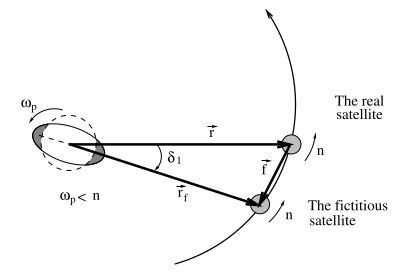
\includegraphics[scale=.8]{shema_planete.png}
		
		\textbf{Figure provenant de l'article illustrant le phénomène des marées}
	\end{center}
	
	Le cœur de l'article \cite{etude} était d'améliorer la modélisation des effets de marées entre une planète et l'un de ses satellites (une application numérique a été faite pour Phobos, une lune de Mars).\\
	
	On se place dans la cadre simplifié de l’article, en supposant l'orbite de Phobos circulaire et équatorial pour pouvoir se mettre dans l'approximation des petits angles notamment.
	
	Le cœur du phénomène de marée provient du décalage entre la position du satellite et la réponse déformée de la planète. En effet, l’attraction gravitationnelle d’un satellite déforme la planète et crée une bosse de marée. Or, le manteau planétaire étant viscoélastique, cette déformation ne se produit pas instantanément mais avec un certain retard. Cette déformation modifie alors le champ gravitationnel exercé par la planète sur le satellite.
	
	Si la bosse se forme en avant du satellite, c'est à dire que la planète tourne plus rapidement sur elle-même que le satellite n'orbite autour d'elle, cette bosse va accélérer le satellite dans le sens de son mouvement et celui-ci va s'échapper de l'orbite à terme (comme la Lune avec la Terre).
	
	Dans le cas contraire, si la bosse est située en arrière du satellite, elle le freine. Il va alors finir par chuter sur la planète comme c'est le cas ici de Phobos.
	
	Pour modéliser ce phénomène, introduisons les grandeurs suivantes (voir schéma ci-dessus). Le satellite situé à la position planétocentrée $\mathbf r$ déforme donc la planète avec un retard $\Delta t$ et un décalage spatial $\mathbf f$ qui correspond à la position d'un satellite fictif par rapport au satellite si la déformation était instantanée. L'angle de retard entre la position réelle du satellite et la position du satellite fictif est noté $\delta$. Nous avons donc avec  $\mathbf r_f$ la position panétocentrée  : 
	\[
	\mathbf r_f=\mathbf r+\mathbf f,
	\qquad
	\mathbf f=\Delta t(\boldsymbol{\omega}_p\times\mathbf r-\mathbf v).
	\]
	Où $\omega_p$ désigne la vitesse de rotation de la planète et $n$ la fréquence orbitale moyenne du satellite, c’est-à-dire sa vitesse angulaire de révolution autour de la planète.
	
	On introduit également la fréquence principale des marées $\chi$. Notons que les marées se produisent deux fois par révolution du satellite. En effet, une seconde bosse de marée se forme également du côté opposé au satellite. C’est pour cette raison que sur Terre les marées hautes dues à la Lune ont lieu environ toutes les $12\,h\,25$, alors que la Terre tourne sur elle-même en $24\,h$ et que la Lune effectue une révolution autour de la Terre en  $27$ jours.
	
	Toutes ces grandeurs sont liées par les relations suivantes dans l’approximation des petits angles. En supposant le triangle formé par $\mathbf r$ et $\mathbf f$ localement rectangle, on obtient :
	
	\[
	\delta \approx \frac{|\mathbf f|}{r}
	=
	\frac{\Delta t}{2}\chi,
	\qquad
	\chi = 2|\omega_p-n|,
	\]
	
	où $\omega_p$ désigne la vitesse de rotation de la planète et $n$ la fréquence orbitale moyenne du satellite, c’est-à-dire sa vitesse angulaire de révolution autour de la planète.
	
	Cette relation est fondamentale pour la suite car elle relie la géométrie du décalage  de marée à la dynamique orbitale du système. En effet, le retard angulaire $\delta$ dépend donc de la fréquence de marée $\chi$ qui est deux fois la différence entre la vitesse de rotation de la planète et de révolution du satellite. Dans la suite, nous verrons également comment ce phénomène est lié à la dissipation d’énergie dans le manteau en introduisant le facteur de qualité $Q$ ainsi que sa relation avec  $\delta$. L’objectif principal de l’article est précisément d’étudier comment cette dissipation dépend de la fréquence des marées et comment cela modifie l’évolution orbitale du satellite.
	
	\section{Facteur de qualité du manteau planétaire}
	
	La réponse viscoélastique interne du manteau aux forces de marée est un phénomène extrêmement complexe faisant intervenir de nombreux mécanismes (dislocations, la diffusion de défauts ponctuels ou encore les interactions entre joints de grains). plutôt que de modéliser l'ensemble de ces phénomènes directement, les planétologues introduisent le paramètre $Q$ ou facteur de qualité qui mesure le taux de dissipation d'énergie dans le manteau de façon analogue au facteur d'amortissement dans l'équation d'un oscillateur harmonique amorti. 
	
	Le facteur de qualité $Q$ dépend de la fréquence $\chi$. D’anciens modèles de marée cités dans l'article supposaient soit un facteur de qualité constant, soit une loi en :
	
	\[
	Q \sim \chi^{-1}.
	\]
	
	Cependant, des mesures expérimentales en laboratoire à basse fréquence ainsi que des observations sismologiques ont progressivement mis en évidence une loi plus réaliste :
	
	\[
	Q \sim \chi^\alpha.
	\]
	
	Dans la plage de fréquences suivantes 
	
	\[
	1\,\text{an}^{-1} \lesssim \chi \lesssim 10^7 \text{ Hz},
	\]
	
	les mesures donnent généralement :
	
	\[
	0.2 \leq \alpha \leq 0.4.
	\]
	
	Cette plage étant très large, elle englobe évidemment la fréquence du phénomène de marée entre Mars et Phobos. 
	
	Cette loi montre que plus la fréquence du phénomène de marée augmente, plus le facteur de qualité $Q$ augmente, soit l'énergie dissipée diminue. Ainsi à haute fréquence c'est le caractère élastique du manteau qui domine face au comportement visqueux car cette réponse visqueuse est très lente.
	
	L’article montre également, par un calcul énergétique et dans l’approximation des petits angles, que :
	
	\[
	Q^{-1}\approx 2\delta.
	\]
	
	Ainsi, lorsque $Q$ augmente, le retard angulaire $\delta$ diminue, ce qui est cohérent avec une dissipation plus faible.
	
	En reprenant la relation :
	
	\[
	\delta \approx \frac{\Delta t}{2}\chi,
	\]
	
	on obtient :
	
	\[
	\Delta t = \mathcal{E}^\alpha \chi^{-(\alpha+1)}
	=
	\mathcal{E}^\alpha \left(2|\omega_p-n|\right)^{-(\alpha+1)}.
	\]
	
	Où le paramètre $\mathcal{E}$ est un facteur dimensionné homogène à un temps permettant de conserver l'homogénéité Il peut être interprété comme un temps de relaxation de la dissipation dans le manteau. 
	
	Ainsi, On obtient des liens étroits entre le retard des marées, la fréquence du phénomène et l’énergie dissipée dans le manteau planétaire. Ce couplage  est au coeur du modèle de l'artilce pour décrire l'évolution de l'orbite de Phobos. 
	
	
	\section{Obtention de l'équation sur le demi-grand axe de Phobos}
	
	L’article établit ensuite l’équation du mouvement du satellite :
	
	\[
	\ddot{\mathbf r}
	=
	-\frac{G(M_0+m)}{r^3}\mathbf r
	+
	\mathbf F_{\text{marée}}.
	\]
	
	Le premier terme correspond à l’attraction gravitationnelle classique du problème à deux corps. Le terme $\mathbf F_{\text{marée}}$ désigne quant à lui la force supplémentaire résultant du potentiel de marée agissant sur le satellite, i.e. l’attraction gravitationnelle exercée par la bosse de marée de la planète sur le satellite. On étudie donc ici l’effet de la déformation de la planète sur le satellite qui a lui-même généré cette déformation. L'articule tronque le développement du potentiel de marée au terme dominant correspondant à la déformation quadrupolaire. On obtient alors la force des marées :
	
	\[
	\mathbf F_{\text{marée}}
	=
	-\frac{3k_2G(M_0+m)mR^5}{r^{10}M_0}
	\left[
	\mathbf -f\,r^2
	-
	2\mathbf r(\mathbf r\cdot\mathbf f)
	\right].
	\]
	
	avec :
	\begin{itemize}
		\item $k_2$ : le nombre de Love quadrupolaire ;
		\item $R$ : le rayon de la planète ;
		\item $M_0$ : la masse de la planète ;
		\item $m$ : la masse du satellite ;
		\item $\mathbf f$ : le retard spatial de la bosse de marée.
	\end{itemize}
	
	
	La dernière étape pour obtenir l’évolution du demi-grand axe orbital de Phobos consiste à projeter cette force sur la composante tangentielle du mouvement du satellite. En effet, c’est cette composante tangentielle de la force de marée qui est responsable des échanges d’énergie et donc de l’évolution du demi-grand axe. 
	
	
	On obtient alors l’équation suivante, que l’on résoudra numériquement dans la suite :
	
	\[
	\frac{da}{dt}
	=
	\frac{6k_2R^5nm\Delta t}{M_0a^4}(n-\omega_p),
	\]
	
	avec pour rappel :
	
	\[
	\Delta t
	=
	\mathcal{E}^{\alpha}
	\left(2|n-\omega_p|\right)^{-(\alpha+1)}.
	\]
	
	\section{Équation sur le demie-grand axe}
	
	\newpage
	
	\part{Résolution numérique}
    \setcounter{section}{0}

    Nous allons nous intéresser à une méthode d'ordre 2 tout aussi simple à implémenter et la comparer avec la méthode d'Euler explicite.
	Nous allons nous intéresser à l'équation suivante : \enc[3cm]{red}{$\dfrac{da}{dt} = f(a)$}\\
	
	avec $f(a) = -\dfrac{6k_2R^5mn(a)}{M_0a^4}\Delta t(a)(n(a)-\omega_p)$, pour $a \in ]0,+\infty[$. Où :
	\begin{center}
		$n(a) = \sqrt{\dfrac{G(M_0+m)}{a^3}}$ \hspace{2cm} $\Delta t_(a) = \mathcal E^{-\alpha}\left(2\abs{n(a)-\omega_p}\right)^{-(\alpha+1)}$\\
		
		avec $\mathcal E > 0$.
	\end{center}
	
	\section{Première propriété de la solution et étude de f}
	
	Soit $a_0 > 0$.\\
    Dans le cas de Phobos, la vitesse angulaire orbitale du satellite est supérieure à la vitesse angulaire de rotation de Mars sur elle-même. On a donc : $n(a_0) > \omega_p$.
	
	\begin{prop}[décroissance]
		Si $n(a_0) > \omega_p$,\\
		\begin{minipage}{18.5cm}
			Alors $\begin{cases}
				\dfrac{da}{dt} = f(a) \\
				a(0) = a_0
			\end{cases}$ possède une unique solution maximale sur un ouvert $U$ tel que $0\in U$ et cette solution est strictement décroissante.
		\end{minipage}
	\end{prop}
	\begin{dem}$ $
		
		\vspace{.2cm}
		
		\begin{minipage}{17.5cm}
			Puisque $n$ est strictement décroissante, continue et que $n(a_0) > \omega_p$, alors il existe $\varepsilon > 0$ tel que pour tout $a \in ]0,a_0+\varepsilon[$, $n(a) > \omega_p$.\\ 
			Ainsi pour tout $a \in ]0,a_0+\varepsilon[$, $\Delta t(a) = \mathcal{E}^{-\alpha}\left(2(n(a)-\omega_p)\right)^{-(\alpha+1)}$ est bien définie, donc $f$ l'est également et est $\mathcal{C}^1$ sur $]0,a_0+\varepsilon[$ comme produit et composition de telles fonctions.\\
			Donc, $f$ est localement lipschitzienne sur $]0,a_0+\varepsilon[$.
		\end{minipage}
		\begin{minipage}{17.5cm}
			Ainsi d'après le théorème de Cauchy-Lipschitz local, le problème possède une unique solution maximale que l'on note $a$, définie sur $]-t_1,t_2[= U$ avec $t_1,t_2 >0$. 
			Puisque $\Delta t(a) > 0$ sur $U$, $f(a)$ est strictement négative sur $U$. Donc $\dfrac{da}{dt}$ est strictement décroissante sur $U$.
			
		\end{minipage}
	\end{dem}
	
	De cela on peut en déduire que $f$ est globalement Lipschitzienne si on ne se rapproche pas de 0 : 
	
	\begin{prop} Soit $0< a_{roche} < a_0$ tel que $n(a_0) > \omega_p$\\
		
		\begin{minipage}{18.5cm}
			$f$ est globalement lipschitzienne sur $[a_{roche},a_0]$ de coefficient de Lipschitz :
			\[L = \underset{a \in [a_{roche},a_0]}\sup\abs{f'(a)}<+\infty\]
		\end{minipage}
		
		\vspace{-.5cm}
		
	\end{prop}
	\begin{dem}$ $
		
		\vspace{.2cm}
		
		\begin{minipage}{17.5cm}
			D'après la preuve précédente $f$ est $\mathcal C^1$ sur $[a_{roche},a_0]$. Donc par l'inégalité des accroissements finis, $\abs{f(x)-f(y)} \leq L\abs{x-y}$ pour tout $x,y \in [a_{roche},a_0]$, avec $L = \underset{[a_{roche},a_0]}\sup\abs{f'}$ qui est fini car $f'$ est continue sur un compact.
		\end{minipage}
	\end{dem}
	
	A partir de maintenant on considère $a$ comme la solution de notre problème sur $I = \R^+\cap a^{-1}([a_{roche},a_0])$.
	
	\section{Méthode d'Euler explicite}
	
	\subsection{Erreur en norme infinie}
	
	La méthode d'Euler explicite est la suivante : $a_{n+1} = a_n + hf(a_n)$ (pour un pas constant).\\
	On sait que cette méthode est d'ordre 1 et on connaît une borne de l'erreur :
	\[
	\abs{a(t_n)-a_n} \leq e^{LT}\frac{M_2T}{2}h
	\]
	où $h = t_{n+1} - t_n$ et $M_2 = \sup \abs{a''} = \sup\abs{f(a)'} = \sup\abs{a'f'(a)} = \sup\abs{f(a)f'(a)}$
	
	\noindent Il faut bien sûr que $f$ soit de classe $\mathcal C^2$ ce qui est le cas si on se place dans les hypothèse de la propriété 2.
	
	Nous allons maintenant estimer l'erreur commise pour savoir à partir de quel pas ce schéma est intéressant pour le cas $\alpha$ = 0.2.\\
	Quelques constantes :
	\[
	\begin{aligned}
		G &= 6.67430\times10^{-11} \hspace{.2cm} m^3kg^{-1}s^{-2}&& \text{ (constante gravitationnelle)}\\
		T &= 3.5\times10^7 \times 365.25 \times 24 \times 3600 \hspace{.2cm} s.&& \text{ (35 millions d'années en secondes)}\\
		M_0 &= 6.4185\times 10^{23} \hspace{.2cm} kg.&& \text{ (masse de Mars)} \\
		m &= 1.06\times10^{16} \hspace{.2cm} kg.&& \text{ (masse de Phobos)} \\
		R &= 3396.2\times10^3 \hspace{.2cm} m.&& \text{ (rayon de Mars)}\\
		k_2 &= 0.169 && \text{ (nombre de Love de Mars)}\\
		a_0 &= 9377\times10^3 \hspace{.2cm} m.&& \text{ (demi-grand axe Phobos)} \\
		\omega_p &= 2\pi/(24.622962\times3600) \hspace{.2cm} rad.s^{-1}&& \text{ (vitesse de rotation de Mars)} \\
		a_{roche} &= 2.2R && \text{ (Distance de Roche (disloquation de Phobos))}
	\end{aligned}
	\]
	
	La valeur de $k_2$ provient de \cite{love}.
	
	\subsubsection{Arrêt de simulation à $a_{min} = a_{roche}$}
	
	Visualisons le graphe de $f'$ :
	\begin{center}
		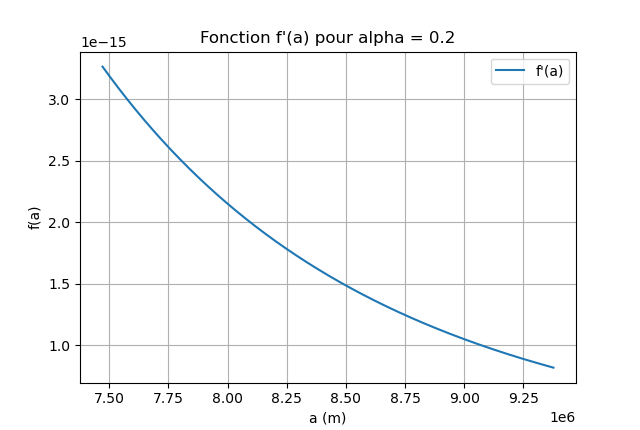
\includegraphics[scale=.5]{f_prim.png}
	\end{center}
	
	On a ainsi que $L \leq 4\times10^{-15}$, de plus $T \simeq 1,2\times 10^{15}$.\\
	Il reste à évaluer $M_2$. On va dans un premier temps faire une première majoration : $M_2 \leq \underset{[a_{roche},a_0]}\sup \abs{f(a)f'(a)}$.\\
	Nous avons donc besoin de la dérivée de $f$ : $f'(a) =
	B_0\, a^{-13/2}
	\left(
	C_1 a^{-3/2} - \omega_p
	\right)^{-\alpha}
	-
	B_1\, a^{-8}
	\left(
	C_1 a^{-3/2} - \omega_p
	\right)^{-(\alpha+1)}$\\
	avec : $\begin{aligned}[t]
		B_0 &= 5,5\dfrac{6k_2R^5m}{M_0}E(\alpha)^{-\alpha}\sqrt{G(M_0+m)}2^{-(\alpha+1)} & \hspace{2cm} & B_1 &= \alpha B_0\\
		C_1 &= \sqrt{G(M_0+m)}
	\end{aligned}$
	
	
	Traçons le graphique de $ff'$ pour ces données :
	
	\begin{center}
		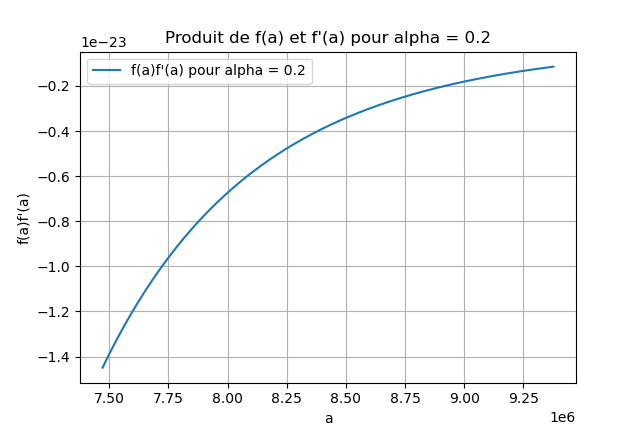
\includegraphics[scale=.5]{ff.png}
	\end{center}
	
	Ainsi $M_2 \leq 1,5\times10^{-23}$. Ainsi $\abs{a(t_n)-a_n} \leq e^{4,5\times1,2\times10^{-9}}\frac{1,5\times1,2\times 10^{15-23}}2 h \leq 2,96\times10^{-7}h$.\\
	
	Ainsi pour une pas de 100 ans : $h \simeq 3,15 \times 10^9$ (donc un nombre total d'environ 350 000), on a : $\abs{a(t_n)-a_n} \leq 931,7 m.$. Le temps d'exécution de l'algorithme est ici d'environ \textbf{2 secondes}.\\
	
	La question qui se pose maintenant est l'ordre de grandeur de la solution, sur quelle plage de valeur va évoluer la solution pour rendre crédible cette erreur. C'est l'objet de la section suivante.\\
	
	Pour $\alpha = 0,2$, on a : $\abs{a(t_n)-a_n} \leq 2,96 \times 10^{-7}h$.\\
	Pour $\alpha = 0,3$, on a : $\abs{a(t_n)-a_n} \leq 2,3 \times 10^{-7}h$.\\
	Et pour $\alpha = 0,4$, on a : $\abs{a(t_n)-a_n} \leq 1,78 \times 10^{-7}h$.
	
	\subsubsection{Arrêt de simulation à $a_{min} = R$}
	
	En effectuant les même calcul pour $a_{min} = R$ (le rayon de Mars), c'est à dire qu'on étudie la chute de Phobos jusqu'à ce qu'elle touche la surface de Mars, la majoration de l'erreur en norme infinie est complètement inutilisable : $\abs{a(t_n)-a_n} \leq 2,7\times10^{196}$.\\
	En pratique la majoration de l'erreur est bien moins grande.\\
	
	Nous avons alors tracé la courbe du coefficient devant $h$ en faisant varier $a_{min}$ (pour un pas de 100 ans) :
	\begin{center}
		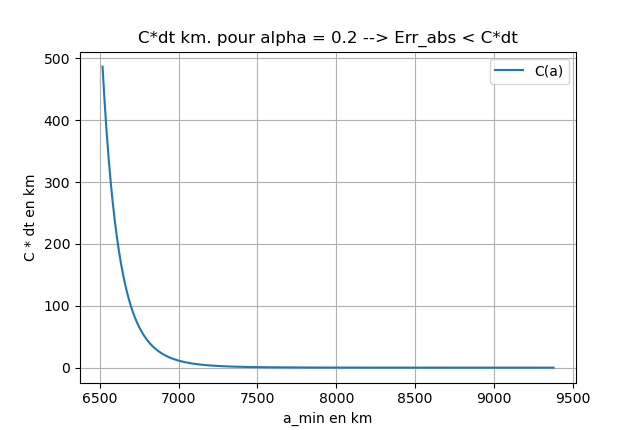
\includegraphics[scale=.5]{sup_err_abs.png}
	\end{center}
	
	La distance à partir de laquelle l'erreur en norme infini est majoré par au maximum 500 km (pour un pas de 100 ans) est : \textbf{6518 km}. Soit à une distance de 954 km en dessous de la limite de Roche situé à $2,2\times R$ de Mars (distance à laquelle le satellite se disloque sous l'effet des forces de gravitation).\\

    En pratique il ne nous semble pas très utile de continuer la simulation en dessous de la limite de roche.
	
	\vspace{-.5cm}
	
	\subsection{Ordre de grandeur de la solution et choix du pas}
	
	Pour $\alpha = 0.2$.	
	Nous allons donc évaluer l'ordre de grandeur de la solution. On note toujours $a$ la solution.\\
	On va chercher à majorer $\abs{a(t_0+h)-a(t_0)}$ par une fonction en $h > 0$.\\
	Effectuons un développement de Taylor-Lagrange en $x_0$ à l'ordre 1 : il existe $\theta_h \in [x_0,x_0+h]$ tel que : 
	\[a(t_0+h) = a(t_0) + ha'(\theta_h) = a(t_0) + hf(a(\theta_h))\]
	Ainsi : $\abs{a(t_0+h)-a(t_0)} \leq \underset{[a_{roche},a_0]}{\sup} \abs f \times h$.\\
	Or $\abs{f} \leq 4.6\times 10^{-9}$.\\
	Finalement $\abs{a(T)-a_0} \leq 4,5\times10^{-9}\times T \leq 4,5\times1.2\times 10^{15-9} = 5,4\times 10^6 m = \mathbf{5400}$ \textbf{km}.\\
	Puisque $a$ est décroissante, on a : \fbox{$a_0-5400 \leq a \leq a_0$}\\
	
	Ainsi l'erreur commise est très faible en comparaison à la plage de valeur que prend $a(t)$ (qui est de l'ordre du millier de km) : $\dfrac{\sup_n abs{a(t_n)-a_n}}{5400} \leq \dfrac{0,9317}{5400} \sim 1,7 \times^{-4} = 0.017 \%$. 
	
	\subsection{Erreur relative}
	
	\vspace{-.5cm}
	
	On en déduit ainsi une majoration de l'erreur relative : $\dfrac{\sup_n\abs{a(t_n)-a_n}}{\sup_n\abs{a(t_n)}} \leq e^{LT}\dfrac{M_2 T}{2(a_0-N_0T)}h $.\\
	Avec $N_0 = \sup\abs{f}$.
	
	\vspace{.2cm}
	
	De même l'erreur relative se comporte bien pour $a_{min} = a_{roche}$ mais pas pour $a_{min} = R$ (rendant cette majoration inutile pour le cas $a_{min} = R$).\\
	
	Pour $a_{min} = a_{roche}$, on a : $\dfrac{\sup_n\abs{a(t_n)-a_n}}{\sup_n\abs{a(t_n)}} \leq 6,6\times10^{-14} h$
	
	\subsection{Comparaison avec Runge-Kutta 45}
	
	Pour pouvoir étudier l'ordre de convergence pratique  et le comparer au théorique, nous avons choisis d'utiliser une méthode déjà implémenté de résolution déjà implémenter dans python : la méthode de Runge Kuta emboîté d'ordre 4 (RK45). A l'aide de cette méthode nous avons calculer une solution que nous considérons comme solution de référence. Et calculons l'erreur de norme infini pour différent pas entre cette solution et la solution obtenue pour ce différents pas par la méthode d'Euler.\\
	Puis nous avons effectuer une régression linéaire pour connaître l'ordre de convergence et le coefficient constant.\\
	Nous avons aussi mesuré, pour ces différents pas, le temps de calcul.\\
	
	\textbf{Tous les graphiques sont ici en échelle log-log.}
	
	\vspace{-.5cm}
	
	\subsubsection{Arrêt de simulation à $a_{min} = a_{roche}$}
	
	\begin{minipage}{10cm}
		
\includegraphics[scale=.5]{erreur_euler.png}
	\end{minipage}\begin{minipage}{10cm}
		
\includegraphics[scale=.5]{temps_euler.png}
	\end{minipage}
	
	Et on retrouve bien l'ordre 1 pour la \textbf{convergence : 0.995}. Et pour le \textbf{coefficient : $\mathbf{3,08\times10^{-16}}$} (soit 100 fois moins que ce qu'on avait calculé). Ce qui confirme nos calculs théorique.
	
	\subsubsection{Arrêt de simulation à $a_{min} = R$}
	
	\begin{minipage}{10cm}
		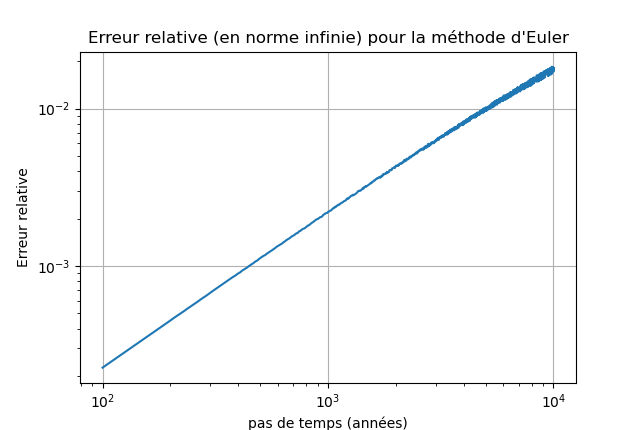
\includegraphics[scale=.5]{erreur_euler_R.png}
	\end{minipage}\begin{minipage}{10cm}
		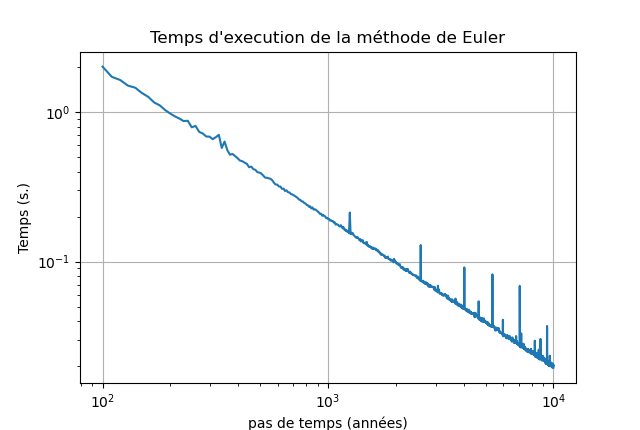
\includegraphics[scale=.5]{temps_euler_R.png}
	\end{minipage}
	
	Et on retrouve bien l'ordre 1 pour la \textbf{convergence : 0.999}. Cependant le \textbf{coefficient : $\mathbf{4,4\times10^{-13}}$} est 1 000 fois plus grand que pour $a_{min} = a_{roche}$ mais reste très correcte.\\
	Nous ne savons malheureusement pas le démontrer.
	
	\section{Graphique de la solution}
	
	\subsection{Nos solutions}
	
	\begin{center}
		
\includegraphics[scale=.8]{sol.png}
	\end{center}
	\begin{center}
		
\includegraphics[scale=.8]{delta.png}
	\end{center}
	
	\hspace{-.8cm}D'après cette simulation, Phobos atteindra la limite de Roche dans 26,2126 millions d'années (pour $\alpha = 0,2$).
	
	\subsection{Les solutions de l'article}
	
	Voici les courbes issu de l'article de Michael Efroimsky1 et Valéry Lainey :
	
	\begin{center}
		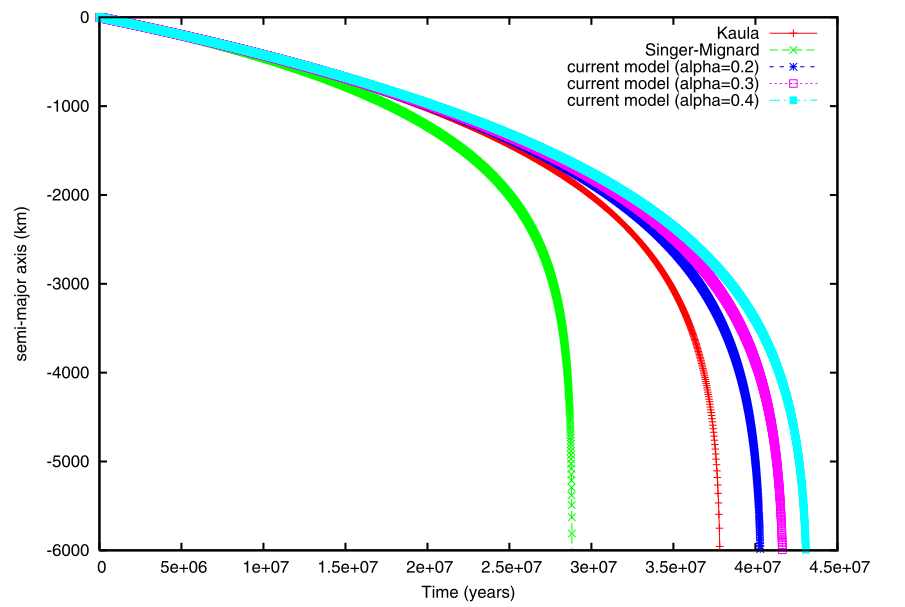
\includegraphics[scale=.4]{article_sol.png}
	\end{center}
	\begin{center}
		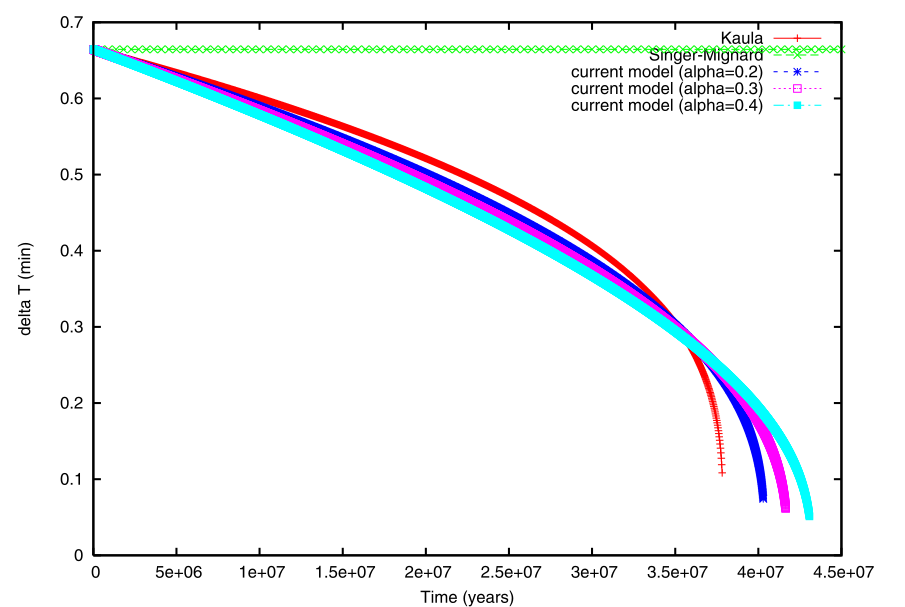
\includegraphics[scale=.4]{article_delta.png}
	\end{center}
	
	On observe que les courbes que nous avons générés décroissent plus rapidement (on observe des différences assez significative), qui sont dû à la valeur de $k_2$ (le nombre de Love), nous avons utilisé une valeur issu d'une étude récente (voir page 4). En remplaçant cette valeur par 0.15 nous obtenons les résultats de l'article : \\


    \vspace{3.5cm}


    \begin{minipage}{10cm}
        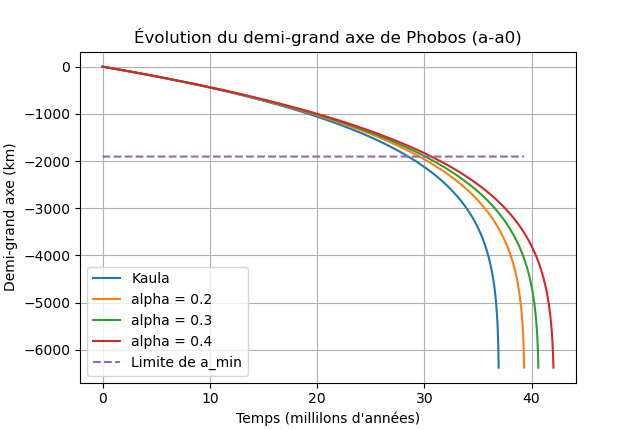
\includegraphics[scale=.5]{sol15.png}
    \end{minipage}
    \begin{minipage}{10cm}
        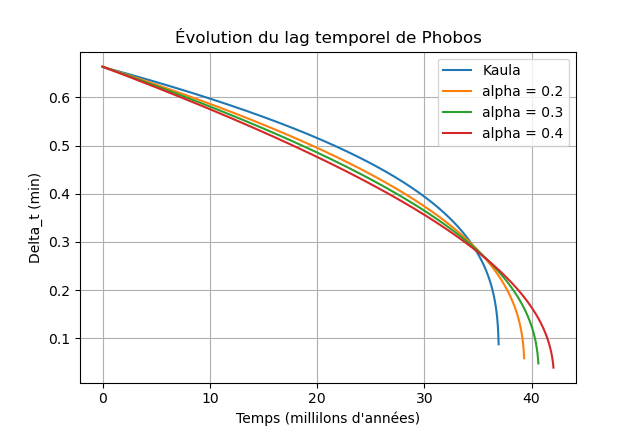
\includegraphics[scale=.5]{delta15.png}
    \end{minipage}
	
	\newpage
	
	\section{Méthode de Heun}
	
	Le schéma de Heun s'écrit ainsi : $a_{n+1} = a_n + \frac h2\left(f(a_n) + f(a_n+hf(a_n))\right)$
	
	\subsection{Résultat théorique}
	
	\begin{enumerate}
		\item \textbf{Consistance :}\\
		On note $\varepsilon_n$ l'erreur de consistance : $\varepsilon_n = a(t_{n+1}) - a(t_n) - \frac h2\left(f(a(t_n)) + f(a(t_n) + hf(a(t_n)))\right)$\\
		
		Effectuons un développement de Taylor-Lagrange à l'ordre 3 :\\
		il existe $\alpha_n \in [t_n,t_{n+1}]$ tel que : $a(t_{n+1}) = a(t_n) + h a'(t_n) + \frac {h^2}2 a^{(2)}(t_n) + \frac {h^3}{6} a^{(3)}(\alpha_n) $\\
		Ainsi $\abs{\varepsilon_n} = \abs{ \frac{h^2}2a^{(2)}(t_n) + \frac{h^3}6a^{(3)}(\alpha_n) + \frac h2 f(a(t_n)) - \frac h2 f(a(t_n) + ha'(t_n))}$.\\
		
		Effectuons un développement de Taylor-Lagrange à l'ordre 2 de $f$,\\ il existe $\beta_n \in (a(t_n),a(t_n) + ha'(t_n))$ : $\begin{aligned}[t]
			f(a(t_n) + ha'(t_n)) &= f(a(t_n)) + ha'(t_n)f'(a(t_n)) + \frac{\left[ha'(t_n)\right]^2}2f^{(2)}(\beta_n)\\
			&= f(a(t_n)) + ha^{(2)}(t_n) + \frac{\left[ha'(t_n)\right]^2}2f^{(2)}(\beta_n)
		\end{aligned}$\\
		
		Ainsi $\abs{\varepsilon_n} = \abs{\frac{h^3}{6}a^{(3)}(\alpha_n) - \frac{h^3}4f(a(t_n))^2f^{(2)}(\beta_n)} \leq h^3\left[\frac{M_3}6 + \frac{N_0^2N_2}4\right]$.\\
		Où $M_k = \sup\abs{a^{(k)}}$ et $N_k = \sup\abs{f^{(k)}}$.\\
		Or $\begin{aligned}[t]
			a^{(3)}(t) = \left(f(a(t))f'(a(t))\right)' &= a'(t)f'(a(t))f'(a(t)) + f(a(t))a'(t)f^{(2)}(a(t)) \\
			&= f(a(t))f'(a(t))^2 + f(a(t))^2f^{(2)}(a(t))
		\end{aligned}$.\\
		Donc $M_3 \leq N_0N_1^2 + N_0^2N_2$. Ainsi $\abs{\varepsilon_n} \leq \dfrac{h^3}{24}\left(4N_0N_1^2+4N_0^2N_2+6N_0^2N_2\right)$.\\
		On pose $C = 4N_0N_1^2+4N_0^2N_2+6N_0^2N_2$.\\
		
		Finalement $\displaystyle\sum_{n=0}^{N-1} \abs{\varepsilon_n} \leq \sum_{n=0}^{N-1} h\frac{h^2}{24}C = \frac{CT}{24}h^2$.
		
		\item \textbf{Stabilité :}\\
		Soit $b_{n+1} = b_n + \frac h2 \left(f(b_n) + f(b_n + hf(b_n))\right) + \mu_n$. Et $h \leq h_max$\\
		$\begin{aligned}
			\abs{a_{n+1}-b_{n+1}} &\leq  \abs{a_n-b_n} + \frac h2\left[\abs{f(a_n)-f(b_n)} + \abs{f(a_n+hf(a_n))-f(b_n+hf(b_n))}\right] + \abs{\mu_n}\\
			&\leq \abs{a_n-b_n} + \frac h2\left[L\abs{a_n-b_n} + L\abs{a_n-b_n + h\left(f(a_n)-f(b_n)\right)}\right] + \abs{\mu_n}\\
			&\leq \abs{a_n-b_n} + \frac h2\left[L\abs{a_n-b_n} + L\abs{a_n-b_n} + L^2h\abs{a_n-b_n}\right] + \abs{\mu_n}\\
			&\leq \abs{a_n-b_n} + hL\abs{a_n-b_n} + \frac{L^2h^2}2\abs{a_n-b_n} + \abs{\mu_n}\\
			&\leq \left(1+ \left[L+\frac{h_{max}L^2}2\right]h\right)\abs{a_n-b_n} + \abs{\mu_n}
		\end{aligned}$\\
		
		Donc d'après le lemme de Grönwall discret : $\abs{a_n-b_n} \leq e^{T\left(L+\dfrac{h_{max}L^2}2\right)}\left[\abs{a_0-b_0}+\displaystyle\sum_{n=0}^{N-1} \abs{\mu_n}\right]$
		
		\item \textbf{Convergence :}\\
		On note $p_m$ la précision machine.\\
		En posant $b_n = a(t_n)$, on a : $\begin{aligned}[t]
			\abs{a(t_n)-a_n} &\leq e^{T\left(L+\dfrac{h_{max}L^2}2\right)}\left[\abs{a_0-a(0)}+\displaystyle\sum_{n=0}^{N-1} \abs{\varepsilon_n}\right]\\
			&\leq e^{T\left(L+\dfrac{h_{max}L^2}2\right)}\left[p_m+\dfrac{CT}{24}h^2\right]
		\end{aligned}$\\
		
		Comme nous codons sur python, nous sommes en double précision : $p_m \leq 3\times 10^{-16}$.
	\end{enumerate}
	
	\textbf{Erreur en norme infinie pour $a_{min} = a_{roche}$}
	
	Effectuons les calculs à l'aide des valeurs données pour les constantes de $f$ :\\
	Pour cela calculons la dérivée seconde de $f$ : $f^{(2)} = B_0\left[f_1+f_2\right] - B_1\left[f_3+f_4\right]$.\\
	$f_1(a) = -\frac{13}2a^{-\frac{15}2}\left(C_1a^{-\frac32}- \omega_p\right)^{-\alpha}$ \hspace{2cm} $f_2(a) = \frac{3\alpha}2 a^{-9}\left(C_1a^{-\frac32}-\omega_p\right)^{-(\alpha+1)}$, avec :\\
	
	$f_3(a) = -8a^{-9}\left(C_1a^{-\frac32}-\omega_p\right)^{-(\alpha+1)}$ \hspace{1.8cm} $f_4(a) = \frac{3(\alpha+1)}2 a^{-\frac{21}2}\left(C_1a^{-\frac32}-\omega_p\right)^{-(\alpha+2)}$
	
	Ainsi \fbox{$\abs{a(t_n)-a_n} \leq 3,28\times10^{-22} h^2$} pour $h \leq 10^{-2}$\\
	
	\textbf{Erreur en norme relative pour $a_{min} = a_{roche}$}
	
	Donc pour $h = 10^{-2}$, on a : $\dfrac{\sup_n\abs{a(t_n)-a_n}}{\sup_n\abs{a(t_n)}} \leq \dfrac{3,28\times10^{-22}}{a_0-N_0T} h^2 \leq 7,2\times10^{-29}$
	
	\textbf{Pour $a_{min} = R$}
	
	De nouveau les valeurs théorique sont complètement aberrantes.
	
	\subsection{Résultat pratique et comparaison avec Euler}
	
	\textbf{Tous les graphiques sont ici en échelle log-log.}
	
	\subsubsection{Arrêt de simulation à $a_{min} = a_{roche}$}
	
	\begin{minipage}{10cm}
		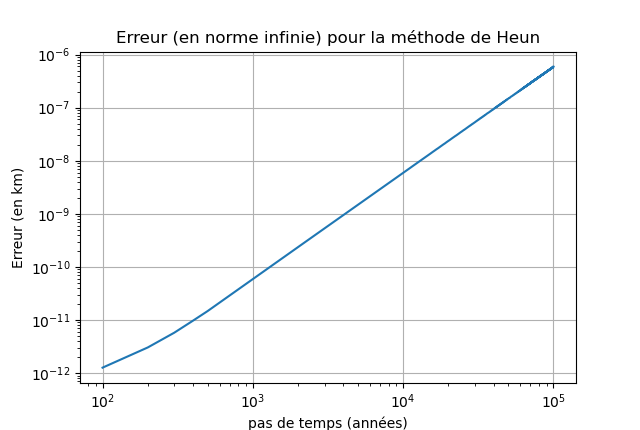
\includegraphics[scale=.5]{erreur_heune.png}
	\end{minipage}\begin{minipage}{10cm}
		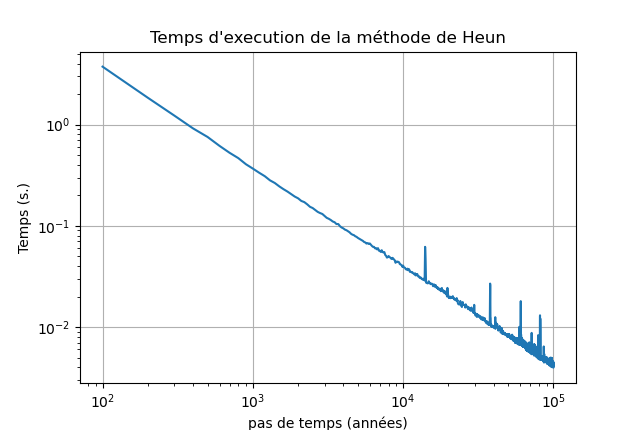
\includegraphics[scale=.5]{temps_heune.png}
	\end{minipage}
	
	\hspace*{-1cm} On retrouve bien l'\textbf{ordre 2 : 1,79}. Et le \textbf{coefficient :} $\mathbf{1,24\times10^{-29}}$ est bien sous celle que nous avions prédite.\\
	
	On remarque quelque chose que l'on aurait pu prédire, la méthode de Heun est moins rapide pour un même pas que celle d'Euler, cela s'explique par le fait que l'on fait plus d'évaluation pour la méthode de Heun que dans celle d'Euler.\\
	Cependant cette différence n'est pas suffisamment significative pour rendre moins intéressante la méthode de Heun, en effet, pour un coût bien moindre (pour le moins fin des pas testé) on est aussi précis que le plus fin des pas testé pour la méthode d'Euler.
	
	\subsubsection{Arrêt de simulation à $a_{min} = R$}
	
	\begin{minipage}{10cm}
		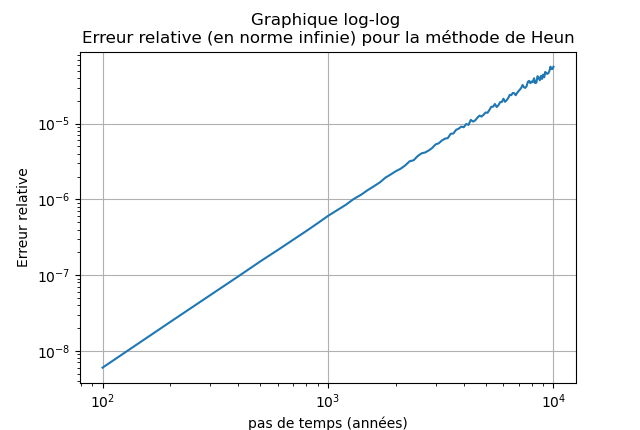
\includegraphics[scale=.5]{erreur_heun_R.png}
	\end{minipage}\begin{minipage}{10cm}
		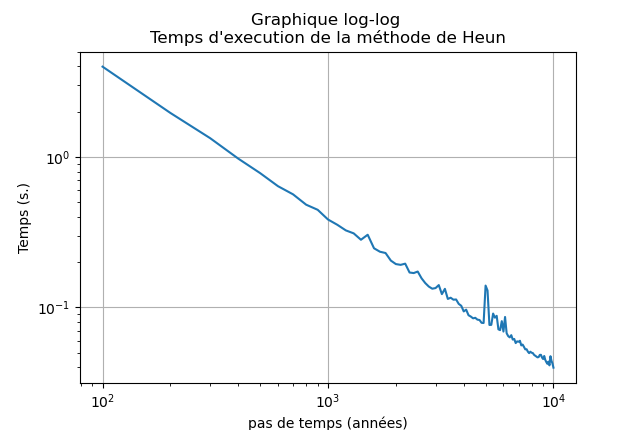
\includegraphics[scale=.5]{temps_heun_R.png}
	\end{minipage}
	
	\hspace*{-1cm} On retrouve bien l'\textbf{ordre 2 : 1,97}. Et le \textbf{coefficient :} $\mathbf{1,32\times10^{-27}}$ est très inférieur au cas $a_{min} = a_{roche}$ mais reste très correcte.\\
	Nous ne savons malheureusement pas le démontrer.
	
    \vfill
	
	\part{Bibliographie}
	
	\begin{thebibliography}{99}	
		\bibitem{etude}
		Efroimsky, Michael et Lainey, Valéry,
		\textit{Physics of bodily tides in terrestrial planets and the appropriate scales of dynamical evolution},
		Journal of Geophysical Research, 2007.
		
		\bibitem{love}
		Yongzhang Yang, Jianguo Yan, Nianchuan Jian, Koji Matsumoto and Jean-Pierre Barriot,
		\textit{Numerical model of Phobos’ motion incorporating the effects of free rotation},
		Arxiv, 2024.		
	\end{thebibliography}
	
	
	
	
\end{document}